\documentclass[10pt,a4paper]{article}
\usepackage[utf8]{inputenc}
\usepackage{amsmath}
\usepackage{amsfonts}
\usepackage{amssymb}
\usepackage{graphicx}
\usepackage{enumerate}
\begin{document}

\section{Set Theory}

To demystify mathematics consider
\begin{enumerate}[(i)]
\item What is a theorem?
\item What is a proof?
\end{enumerate}
What if we don't know the answer?

To begin we need
\begin{enumerate}[(a)]
\item an example(s)
\item a nearly related concept
\end{enumerate}


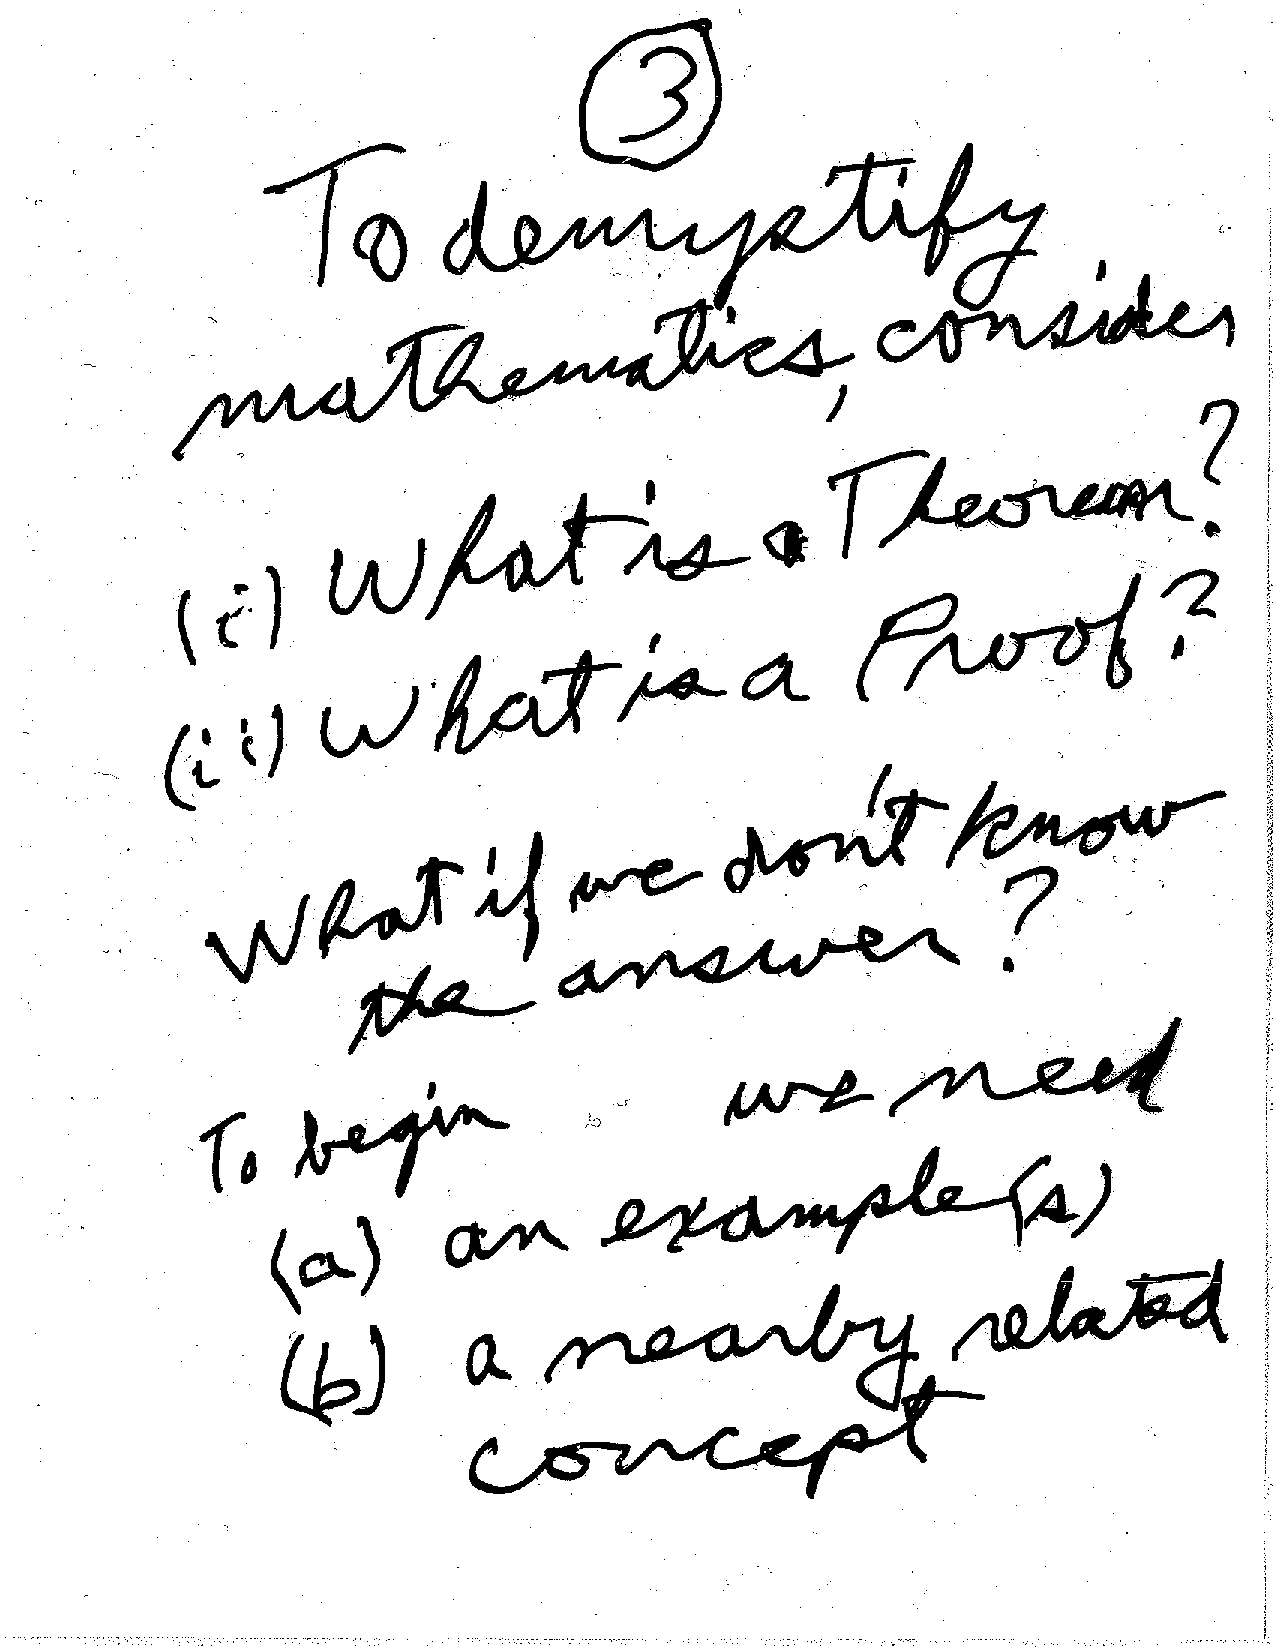
\includegraphics[scale=.5]{Pages/ST_3}

\newpage

Related Concept: Greek Syllogism

\underline{example:}
\begin{enumerate}
\item All men are mortal.
\item Socrates is a man.
\item Therefore, Socrates must die. 
\end{enumerate}

To analyze, recast in set theoretic terms via Venn Diagram.

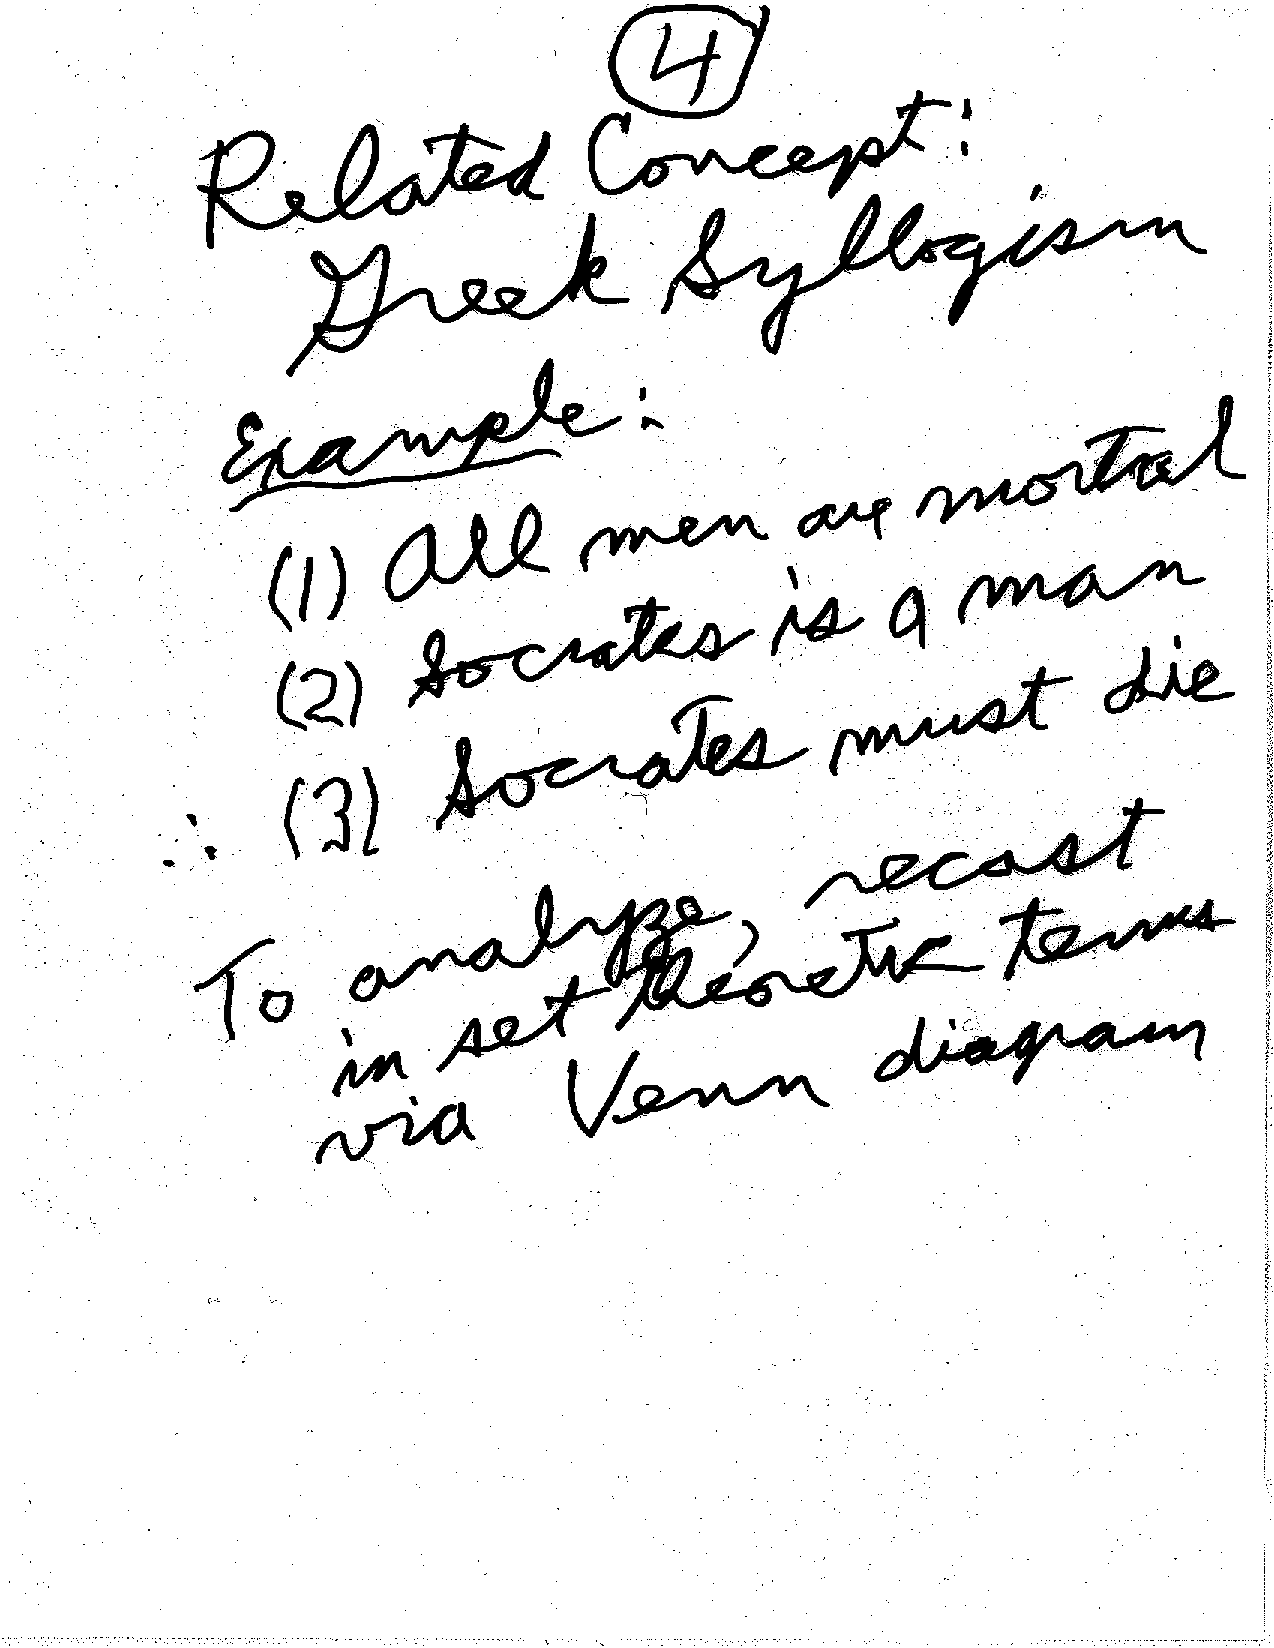
\includegraphics[scale=.5]{Pages/ST_4}

\newpage

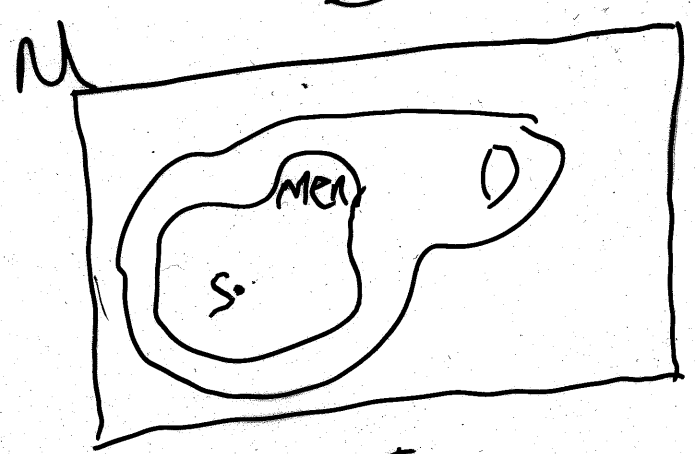
\includegraphics[scale=.2]{Pages/ST_5_im1}

$S$: Socrates\\
$M$: Set of Men\\
$D$: Things that will die\\
$\mathcal{U}$: Things on Earth

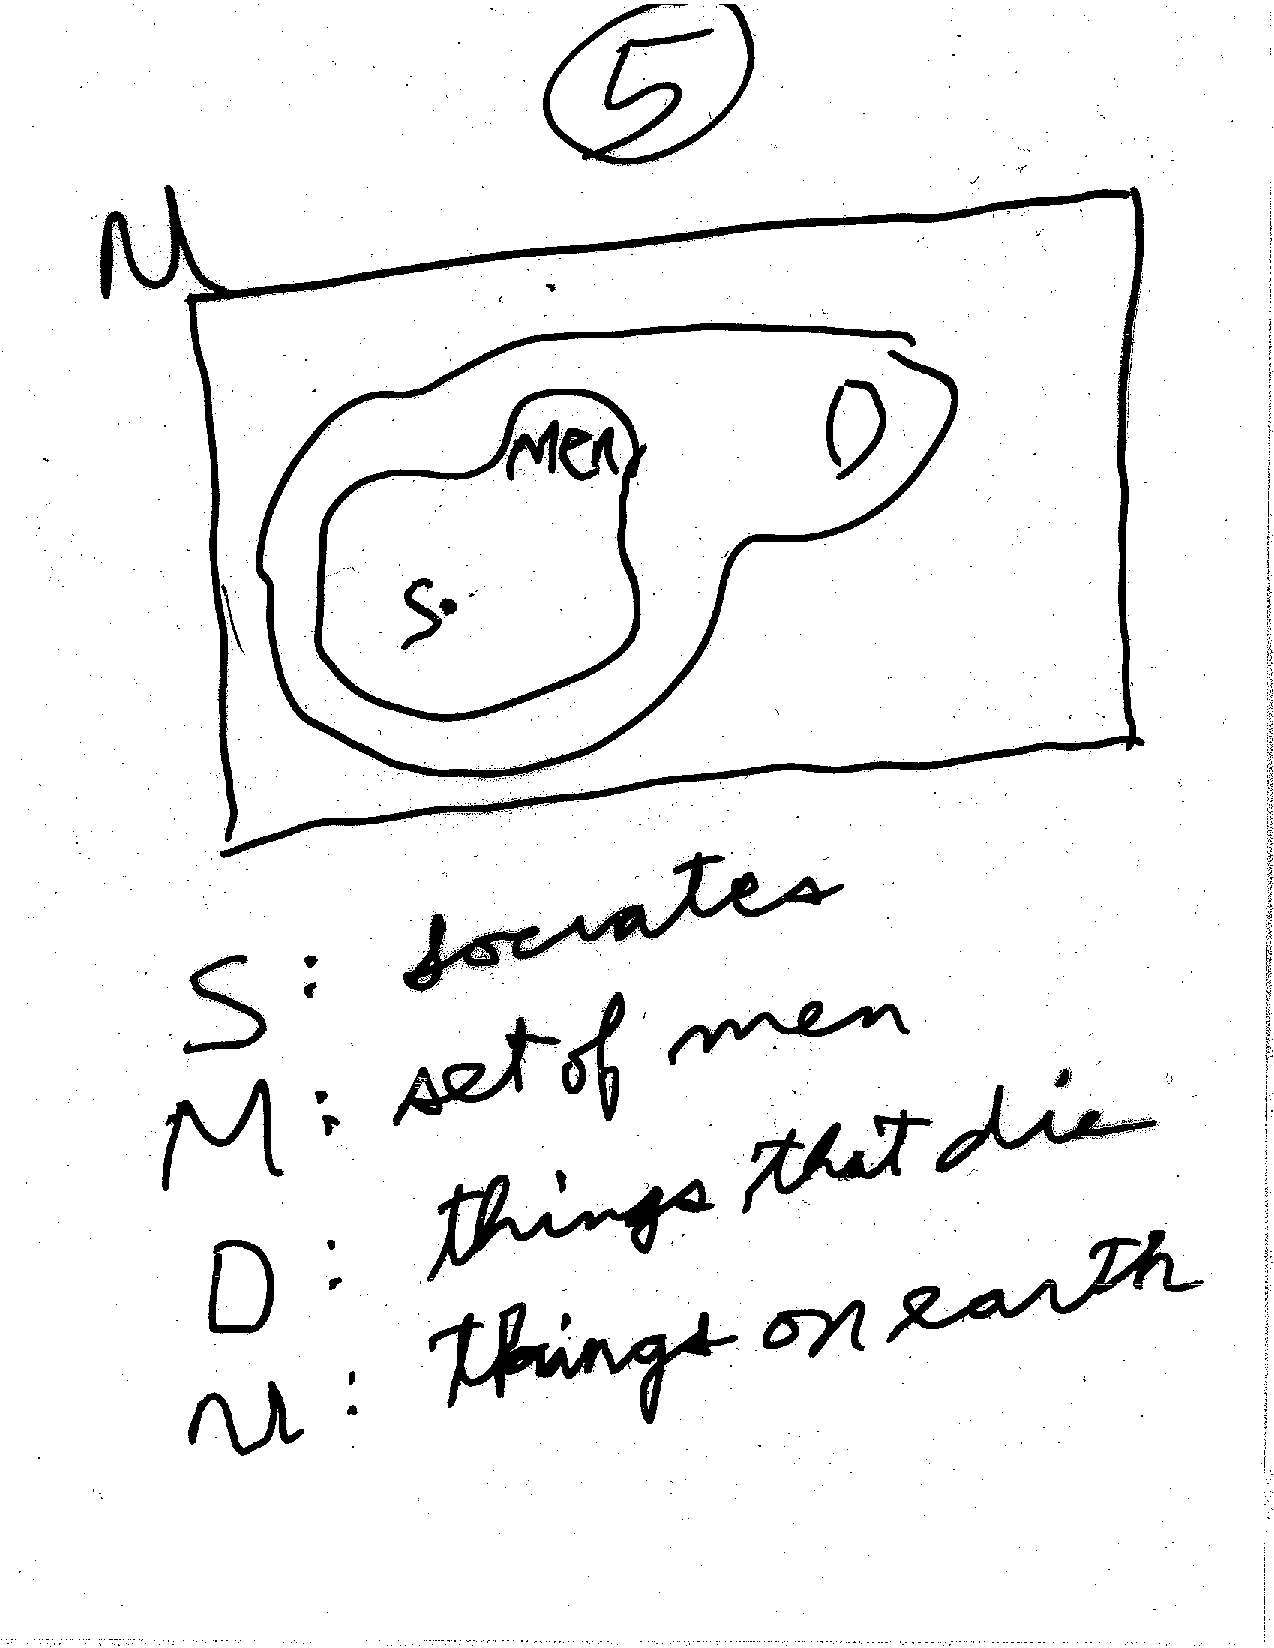
\includegraphics[scale=.5]{Pages/ST_5} 



%Zack: Pages 6,7,8,19,20

%Jack: 21, 9, 10, 11

%Koka: Pages 13, 13A, 22 ,22A, 22B


\section{Generate $\mathbb{N}$}


%Ruth: Pages L4A-L4G




\section{From $\mathbb{Z}$ to $\mathbb{R}$ via ordering}
%Jazz: ZR1-ZR5

%Kyler: ZR6 - ZR10

%Preethika: ZR11-ZR14


\section{Sequence and Limits}

%Aaron: First 2 pages and 48-50

%Hamza: 51-52B

\section{Limit and Convergence}

%Joe: 50-51
\newpage

z

\underline{Finding Limits and Proving Convergence}

\underline{Example 1} $\frac{lim}{n \rightarrow \infty}  \frac{1}{n^2} = 0$

\underline{Example 2} $\frac{lim}{n \rightarrow \infty} \frac{3n +1}{7n-4} = ?$

\underline{Example 3} $\frac{lim}{n \rightarrow \infty} (1+ \frac{1}{n})^n = ?$

\underline{Example 4} Find $\frac{lim}{n \rightarrow \infty} (\sqrt{n+1}-\sqrt{n})$

HW suppose $a_n \rightarrow a > o$

Prove: $\sqrt{a_n} \rightarrow \sqrt{a}$

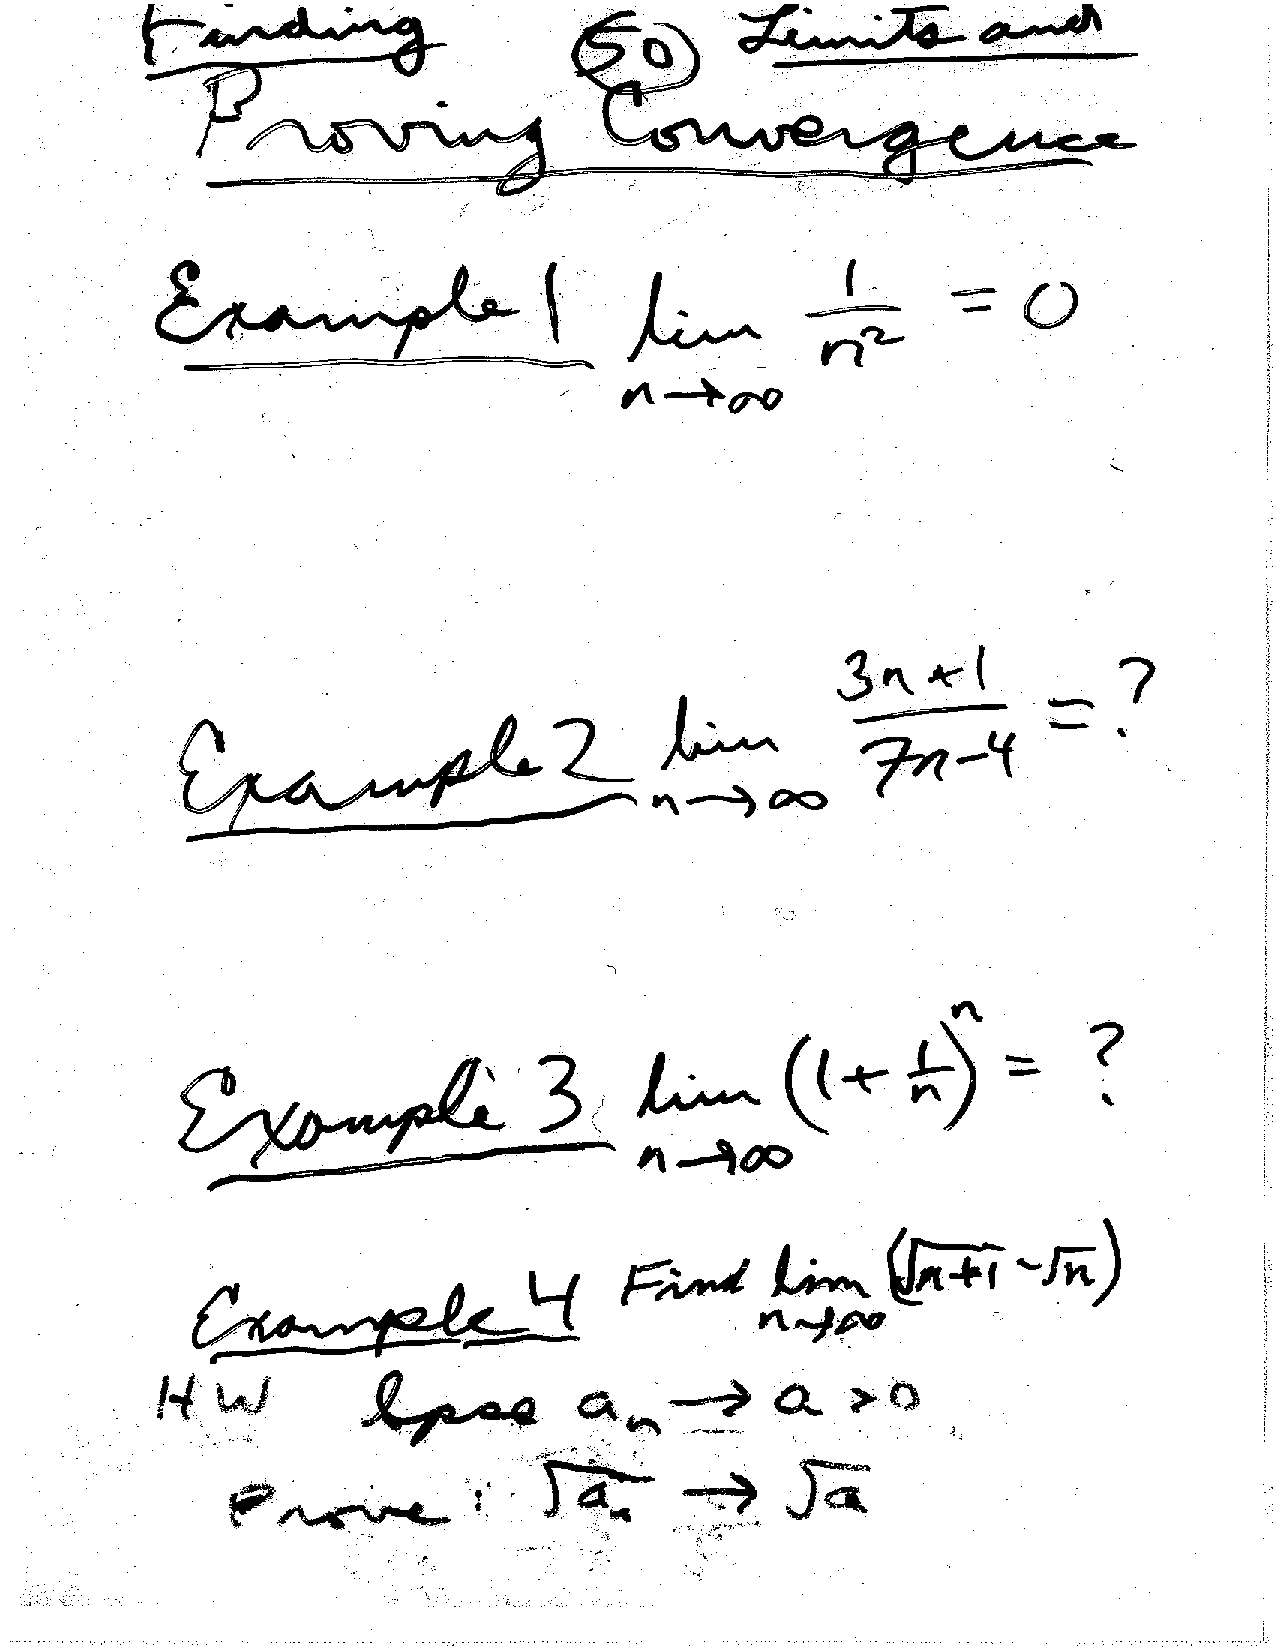
\includegraphics[scale=.5]{Pages/LC_50}

\newpage
\underline{Properties of Limits}

\underline{Theorem} Suppose $a_n \rightarrow a$ and
 
$b_n \rightarrow b$. Then

$a_n + b_n \rightarrow a + b$

(and $\lambda a_n \rightarrow \lambda a$)

and $a_n b_n \rightarrow a \cdot b$

\underline{Theorem} of $a_n \rightarrow a \neq o$,

then $\frac{1}{a_n} \rightarrow \frac{1}{a}$

\underline{Corol} if $a_n \rightarrow a$ 

and $b_n \rightarrow b \neq 0$ then 

$\frac{a_n}{b_n} \rightarrow \frac{a}{b}$

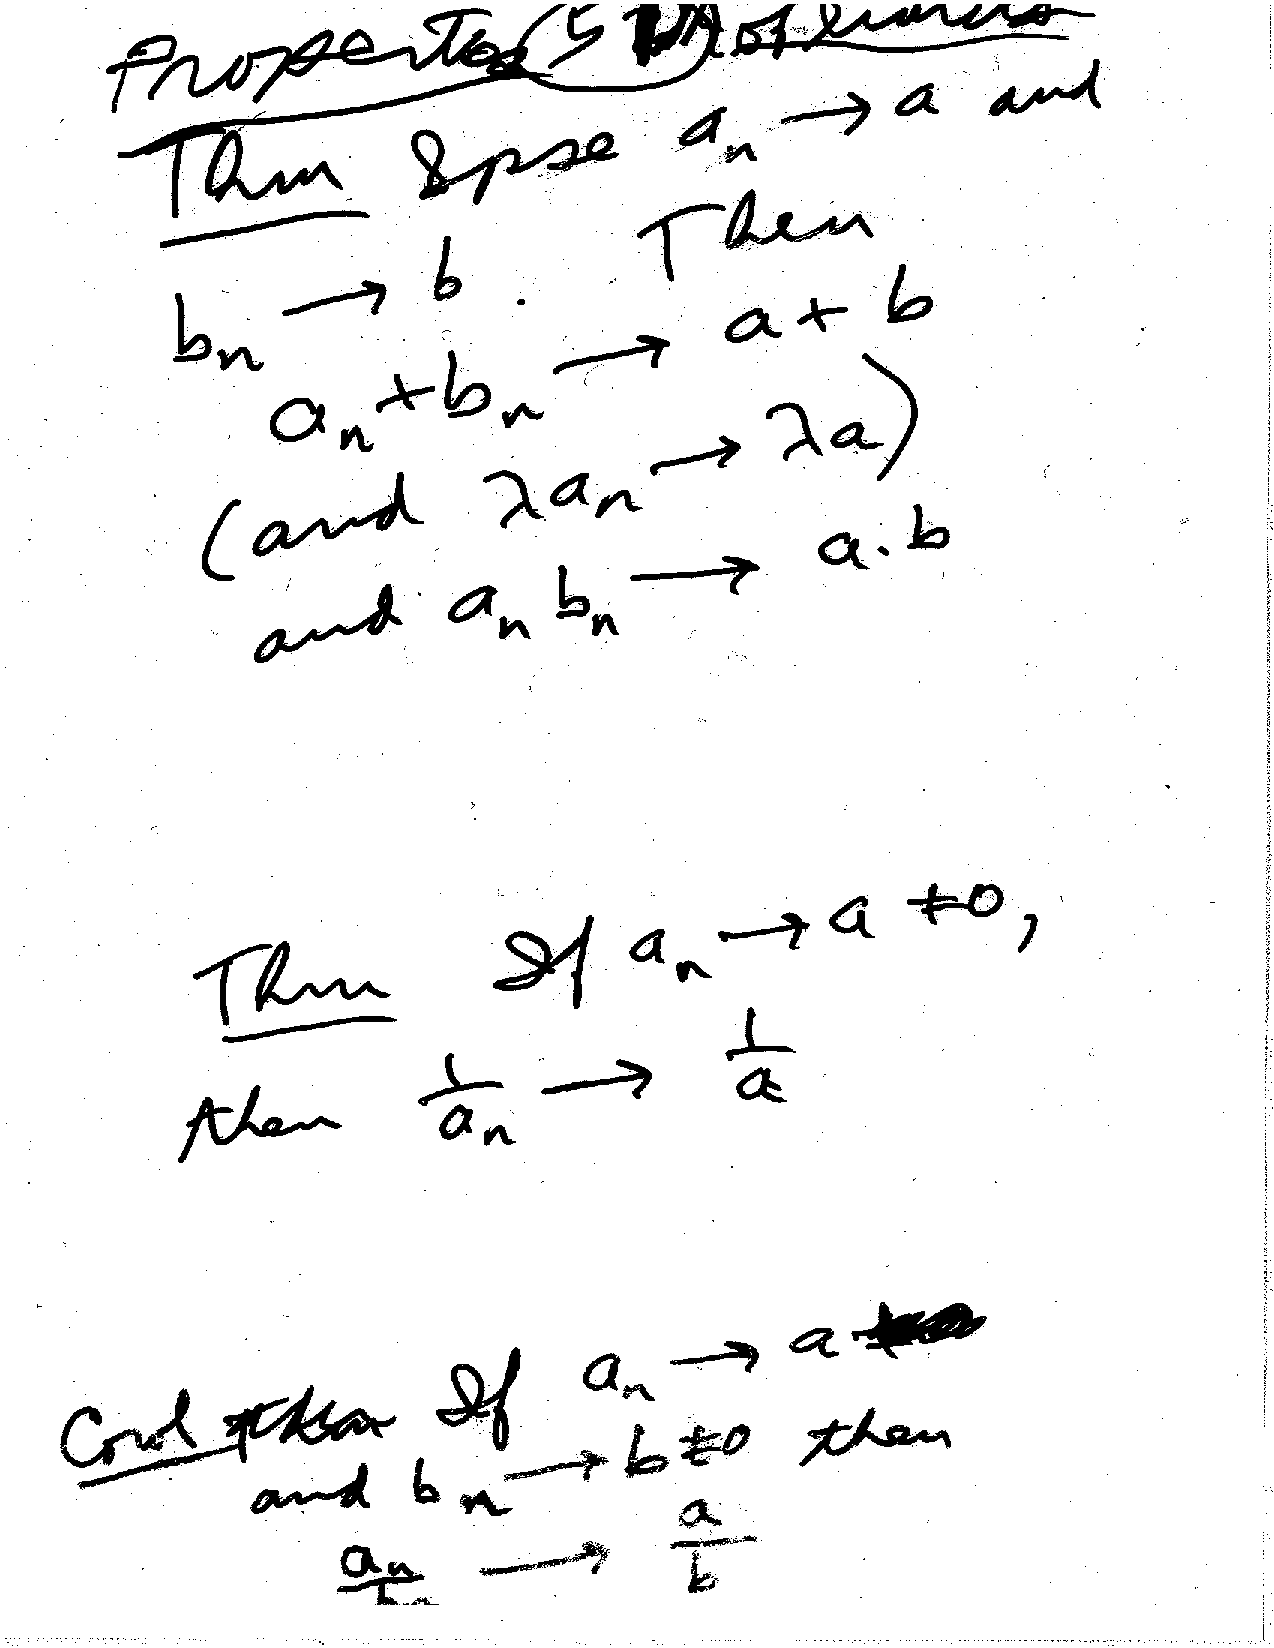
\includegraphics[scale=.5]{Pages/LC_51}

%Quinten: 52-53

%Farishta: 53A-54A

\section{Infinite Series}

%Sukhreet: IS1 - IS 7

%Matthew: IS8 - IS15

%Will: IS16 - IS23

%Rebecca: IS24 - IS32

%Maady: IS33 - IS42

\section{Metric Spaces Part 1}

%Travis: M1 - M5

%Jerome: M6- M10



\section{Metric Spaces Part 2}


%Bryant: M1-M7

%Reshma: M8-M14

%Ethan: M15-M21





\end{document}